\documentclass[conference]{IEEEtran}
\IEEEoverridecommandlockouts
% The preceding line is only needed to identify funding in the first footnote. If that is unneeded, please comment it out.
\usepackage{cite}
\usepackage{amsmath,amssymb,amsfonts}
\usepackage{algorithmic}
\usepackage{graphicx}
\usepackage{textcomp}
\usepackage{xcolor}
\usepackage{url}
\usepackage[section]{placeins}
\def\BibTeX{{\rm B\kern-.05em{\sc i\kern-.025em b}\kern-.08em
    T\kern-.1667em\lower.7ex\hbox{E}\kern-.125emX}}
\begin{document}

\title{Sentimental Analysis of Amazon Reviews\\
}

\author{\IEEEauthorblockN{Sagar Punn}
\IEEEauthorblockA{\textit{Computer Science} \\
\textit{Ryerson University}\\
Toronto, Canada \\
sagar.punn@ryerson.ca}
\and
\IEEEauthorblockN{Adam Sorrenti}
\IEEEauthorblockA{\textit{Computer Science} \\
\textit{Ryerson University}\\
Toronto, Canada \\
adam.sorrenti@ryerson.ca}
\and
\IEEEauthorblockN{Eisa Keramatinejad}
\IEEEauthorblockA{\textit{Computer Science} \\
\textit{Ryerson University}\\
Toronto, Canada \\
eisa.keramati@ryerson.ca
}
}

\maketitle

\begin{abstract}
Final report of an application level project using machine learning classification algorithms in sentimental analysis and comparing results between algorithms. 
\end{abstract}

\begin{IEEEkeywords}
NLP (Natural Language), Natural Language Toolkit (NLTK), BOW (Bag of Words), TFIDF (Term Frequency Inverse Document Frequency), Negation (NEG), K Nearest Neighbours (KNN), Principal Component Analysis (PCA), Stemming, Filtering
\end{IEEEkeywords}

\section{Introduction}
Sentiment analysis is the interpretation and classification of text based data. The point of this analysis is to categorize each data-point into a class that represents it’s quality (positive, negative, etc). Sentiment analysis focuses on polarity, emotions and intentions of authors. Classic sentiment analysis consists of the following steps: preprocessing, training, feature extraction and classification. The method used in this paper will follow the classical approach while applying sentimental analysis on Amazon reviews.

\subsection{Challenges}\label{AA}
Due to the nature of the Amazon reviews, the five star rating system is a good, but not perfect, indication of the positivity/negativity sentiment of reviews. Outliers become apparent when looking at the three star reviews.These reviews were ultimately considered as inherent noise of sentiment analysis of Amazon reviews. The second challenge which is common with most NLP-related projects, is having a huge body of features causing high dimensionality. When dealing with text data, and using the common preprocessing models such as, bag of words or TFIDF, where each feature represents a word, this raises questions about their relevance. The main problems faced was finding solutions and compromises for the dimensionality of our feature set.

\subsection{Prior work}
Reference [1], is an example of prior work performed on similar Amazon reviews looking at sentiment analysis. Some major differences in methodologies include: First, in the processing of the dataset, despite the original dataset being unbalanced, the prior project the data was intentionally balanced so that the number of positive reviews are equal to the negative ones. For the methodology discussed here, the data was kept unbalanced in order to more accurately train our model in accordance with the real-world distribution of review sentiment. The accuracy levels achieved here actually surpassed that seen in the prior works by approximately 15\% while maintaining a model true to the practical zeitgeist of Amazon review sentiment.

\subsection{Overview}
Elaborating further on the rest of the project, different methods of text preprocessing such as pure BOW, TFIDF, stemming and filtering were used. The project started with a simple BOW representation, which provided more than 62 thousand features and finished off with a TFIDF stemmed and filtered version that reduced the number of features to only eight-hundred (an approximately 98.7\% reduction). The main machine learning algorithms used were, multinomial naive bayes, logistic regression, support vector machines, k-nearest neighbours clustering algorithm and decision trees. For implementation of these algorithms, the python scikit learn and NLTK libraries were mainly used. Aside from attaining high levels of accuracy and performant precision/recall in almost all of the methods and variations, one of the main achievements of this project was after revising the preprocessing model and reducing the number of features while maintaining or improving performance metrics within margin of error. Furthermore, removing the three star reviews significantly improved performance metrics. This post-processing step supported the hypothesis that three star reviews acted as an inherent noise and made it difficult for our model to learn the binary decision bound despite the extensive progress made on feature selection and model tuning.


\section{Problem Statement}

	More rigorously, the problem faced implied classifying an Amazon review with a positive or negative sentiment, exclusively. For example, given the following review: 'Super comfortable and extremely lightweight. Great for crossfit!' Using machine learning and natural language processing is a must to identify whether the review implies a positive or negative sentiment. This entails breaking each review down into its most relevant components and then applying machine learning techniques to assign weighted sentiment scores to the samples. By the implementation of data processing techniques, which will be discussed in more detail later, the example review given previously was tokenized into the following list of sentimentally relevant words: [super, comfort, extrem, great]. Training your model on a refined list of the most relevant tokens is central to the problem of sentiment analysis and will result in a more robust model.
	
\section{Dataset}

	The dataset [2] used includes 233.1 million Amazon reviews spanning from May 1996 to October 2018 and over a total of thirty unique e-commerce categories. For the purpose of this project, the approximately 140 thousand reviews were randomly sampled from each category proportional to the size of that category. This allowed for an optimal representation of the dataset within reasonable computational restraints. The resulting dataset is unbalanced in favour of positive reviews and the decision was made to preserve this aspect of the data to better represent the nature of sentimental analysis of Amazon reviews. Although, preserving the unbalanced nature of the data implied taking precautions when analysing performance metrics which will be noted later. Furthermore, the structure of the dataset followed the form of {‘Summary and Review’, ‘Rating’, ‘Overall’}, where ‘Summary and Review’ is the title of a given review concatenated with the full review text, ‘Rating’ is either zero or one corresponding to positive or negative sentiment, respectively, and where ‘Overall’ is the original star rating from one to five. How exactly the ratings were assigned to the sample will be discussed in further detail in the methods and models section.

	Following a BOW and TFIDF approach, the initial dimensions of the features was approximately 64 thousand degrees, well out of the acceptable range and feature selection techniques were employed to refine this. Of course, we labelled the data with a binary, positive or negative sentimental value, in accordance with the provided star ratings from the source.


\section{Methods and Models}

\begin{figure}[htbp]
\centerline{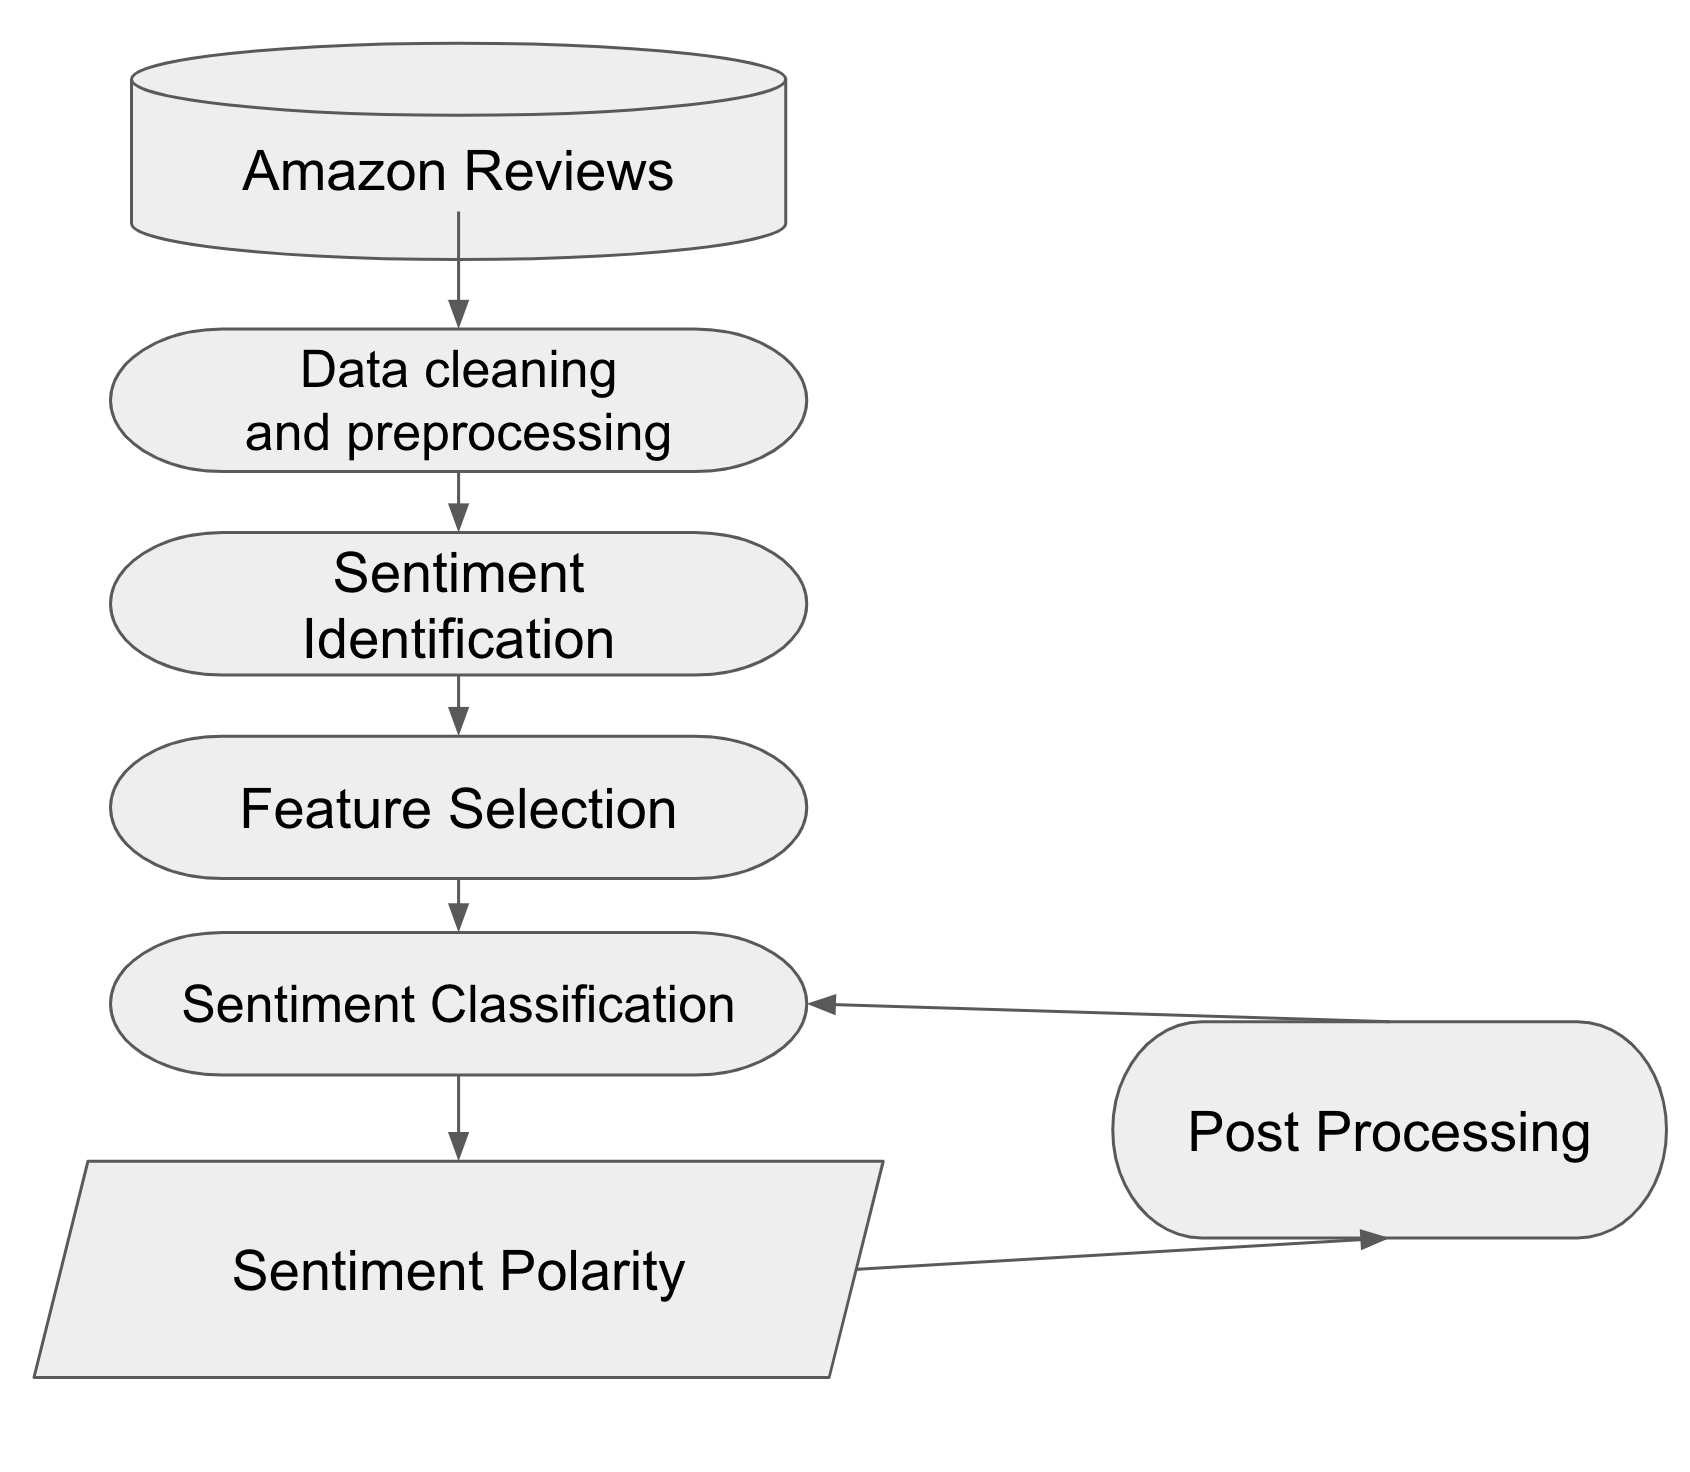
\includegraphics[width=0.8\columnwidth , height=6cm]{flowchart.png}}
\caption{Sentimental analysis process.}
\label{fig}
\end{figure}
\FloatBarrier
Fig. 1 is the sequence of steps that were taken in order to tackle classification of sentiments. Initially preprocessing is applied on raw dataset after which sentiment labelling/identification took place. Then a variety of experimentation is done to get multiple versions of the dataset to put inside the model. After each iteration of dataset variation post processing methods were applied in order to gain better results and then the process was repeated on every dataset variation.

\subsection{Data Preprocessing}
From the original dataset only review text (concatenation of summary and body text) and overall ratings were considered. Since our methodology is concerned with binary classification, overall ratings (from 1-5) were converted to 0 (1 and 2 star) or 1 (4 or 5 star) representing negative or positive sentiment respectively. For 3 star reviews ambiguity arises in terms of sentiment and since the goal of this report is to apply binary classification methods, use of neutral class is not utilized, hence 3 stars are given 0/1 label randomly.
\subsection{Features Selection}
In this case, BOW and TFIDF approach is employed where, for BOW, the dataset is converted into a matrix where features are all words in our dataset’s dictionary and row contains word frequency in a review. In contrast, for each word within a review, TFIDF contains normalized count. For both BOW and TFIDF, some baseline conditions were set where former removes stop words and latter only considers words with a minimum of 50 document frequency. These two baseline approaches are applied on top of the following variations of the dataset:

\subsubsection{Regular}
This is untouched review without any filtering applied.
\subsubsection{Stemmed}
In this case, Porter Stemmer is used to stem original review text where stemmer removes morphological affixes from words, leaving only the word stem[4]. After which BOW and TFIDF are applied.
\subsubsection{Filtered}
Each review is filtered to only contain positive and negative words using opinion lexicon list [5]. Before employing the filtering process, reviews are passed through Mark Negation method [6] which appends NEG on words between a negation and punctuation mark. Furthermore, all words with NEG are considered as one single word in order to reduce noise. This process significantly reduced the amount of features and BOW and TFIDF are applied at the end.
\subsubsection{Filtered Stemmed}
Here first reviews are filtered (as explained above) and then stemmed. Finally BOW and TFIDF are applied.

The reason these variations were created was due to large amounts of features produced by the regular model where a lot of noise seems to be generated (discussed in the results section).  Our hypothesis is that only positive/negative words have an effect on the overall sentiment of the review, therefore filtering was done. Also, stemming is employed where this report hypothesized that reducing multiple words to their root element would help in reduction of features and removing noise.

\subsection{Dataset Split}
Dataset is split into 60:20:20 ratio where training accounts for 60\% and both validation and testing account for 20\%. This was done to ensure hyper-parameters of the models are tuned based on valid set results and final accuracies are based on test set. Furthermore, before making final predictions on the test set, the training and validation set were combine in order to take advantage of the full 80\% of allocated training data.

\subsection{Models}
Following are the classification models that were used in this report:
\subsubsection{Logistic Regression}
Baseline version with max iterations set in range 1000-10000 in order for model to converge.
\subsubsection{Multinomial Naive Bayes}
Baseline version used.
\subsubsection{Support Vector Machine}
Baseline version used with max iterations set in the range of 1000-20000 and, if failed to converge, the dual formulation parameter was set to false.
\subsubsection{K Nearest Neighbours}
Three variations of this model were used where the number of neighbours was set to 1, 3, and 5.
\subsubsection{Decision Trees}
First baseline version is employed after which criterion of split is set to entropy with depth of tree being 3. Last variation just consisted of the depth of the tree set to 5. 


\subsection{Post Processing}

After implementing the main variations and algorithms, a method was developed to capture the mislabelled reviews. By looking at some of the mislabelled reviews it was found out that the majority of them consisted of former three star reviews which were randomly assigned a positive/negative label during the preprocessing stage. For instance a review that was written with satisfaction and was overall a positive one was predicted correctly however in the preprocessing stage randomization step label it negative review. After this observation we had a hypothesis that the three star reviews were more noisy than we thought and have almost no contribution to the learning process, and the Extreme version was devised. In the extreme version training data only consists of one and five star reviews. By omitting the rest of the reviews the amount of noise in the training process is minimized and only the reviews that were surely positive or negative were given to the model. 

\subsection{Performance Metric}
The metrics used implements functions for assessing prediction error/success and visualizations to better identify upward performance trends while training. Again, all tuning is performed in relation to the validation set to ensure the integrity of the models predictive capabilities. The following performance metric were used and helped guide next steps:
\begin{enumerate}
\item Accuracy Score
\item Precision \& Recall
\item F1 Score
\end{enumerate}
Due to the unbalanced nature of the dataset, with reviews tending to a positive sentiment in general, special attention was paid to the metrics resulting from precision and recall. Accuracies, while useful for showing final performance, did not show the whole picture when tuning models and hyper-parameters. A precision-recall curve also showed the trade-off between precision and recall for different thresholds. A high area under the curve represents both high recall and high precision, where high precision relates to a low false positive rate, and high recall relates to a low false negative rate. Whereas, F1 score can be interpreted as a weighted average of the precision and recall, where an F1 score reaches its best value at one and worst score at zero.

\section{Results and Discussions}
\begin{figure}[htbp]
\centerline{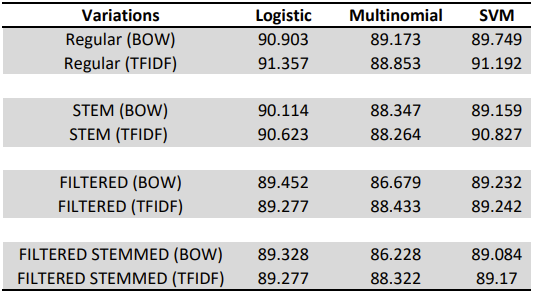
\includegraphics[width=0.9\columnwidth , height=4cm]{test-prediction-main.png}}
\caption{Accuracies in percent of test set predictions.}
\label{fig}
\end{figure}

\begin{figure}[htbp]
\centerline{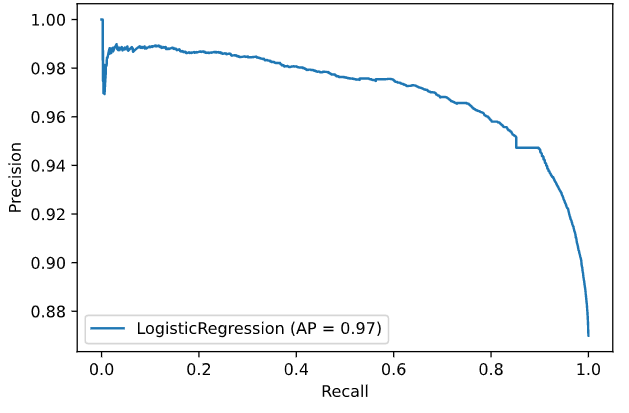
\includegraphics[width=0.9\columnwidth]{precision-recall.png}}
\caption{Precision-Recall curve for logistic regression on Filtered-Stemmed-BOW samples.}
\label{fig}
\end{figure}
\FloatBarrier
In the beginning stages BOW or TFIDF models were mainly used to pre-process the text and to vectorize it. This led to a huge number of features and made the dataset high dimensional. As the model was trained on this data, we achieved high accuracy on the training set but the accuracy on the validation and the testing set were lower. This difference suggested over fitting. Since the model kept over fitting to the training data, it was clear there was an unnecessary amount of complexity, therefore variance. This was most significant in the baseline version of SVM, KNN and Decision Tree with slightly less variance in Logistic with BOW without any filtering. 


\begin{figure}[htbp]
\centerline{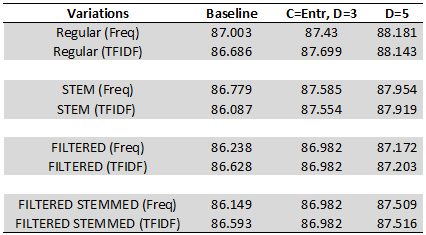
\includegraphics[width=0.9\columnwidth]{descision-tree-predition.png}}
\caption{Accuracies in percent of test set for a decision tree classifier.}
\label{fig}
\end{figure}

\begin{figure}[htbp]
\centerline{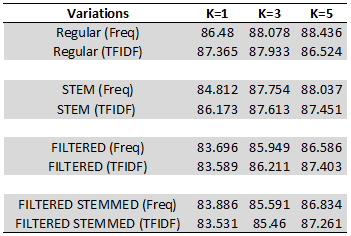
\includegraphics[width=0.9\columnwidth]{knn-prediction.png}}
\caption{Accuracies in percent of test set for a KNN classifier.}
\label{fig}
\end{figure}
\FloatBarrier
For KNN and Decision Tree, after tuning hyper-parameters, variance was reduced regardless of the kind of dataset used. Similarly there was high variance present in the regular BOW dataset throughout Logistic, Multinomial NB and SVM, but after applying filtering process, variance dropped significantly, however, at the cost of slight reduction in accuracies. 

This high variance might have been caused by the high number of features. After implementing the filter and stemmed version of the previous preprocessing stage which lowered the number of features to 1.3\% of the original number, the complexity of the model decreased and the results stated that the model was closer to the goal of having low bias and low variance. 

\begin{figure}[htbp]
\centerline{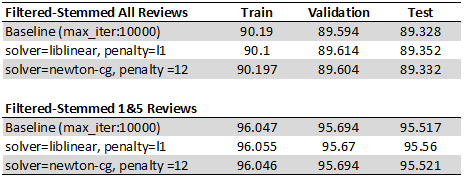
\includegraphics[width=0.9\columnwidth]{one-five-predictions.png}}
\caption{Accuracies in percent of train/valid/test sets for a modified logistic regression classifier on one-five star reviews.}
\label{fig} 
	
\end{figure}
\FloatBarrier
Noise trade-off was also an issue, as the first set of results were reviewed, a post-processing part was implemented in which mislabelled reviews were studied. This study revealed that a huge number of mislabelled reviews were those that originally had 3 star ratings. Since in the preprocessing stage each 3 star review was assigned a random label of positive or negative, In a lot of cases the model had predicted a 3 star rating review written with overall positivity and content to be a positive review but since it was randomly assigned a false truth label of negative, it was counted as an error. This observation suggested that the model could not fully rely on the 3 star reviews on the training and contributing more to the noise. In the next stage the 3 star reviews were removed from the dataset and only the one and five star reviews were passed on to the training stage. This decision to only look at the extreme sides of each end (1 and 5 stars) provided a higher accuracy (cite the table with extreme) that proved our hypothesis about the three star reviews.

\begin{figure}[htbp]
\centerline{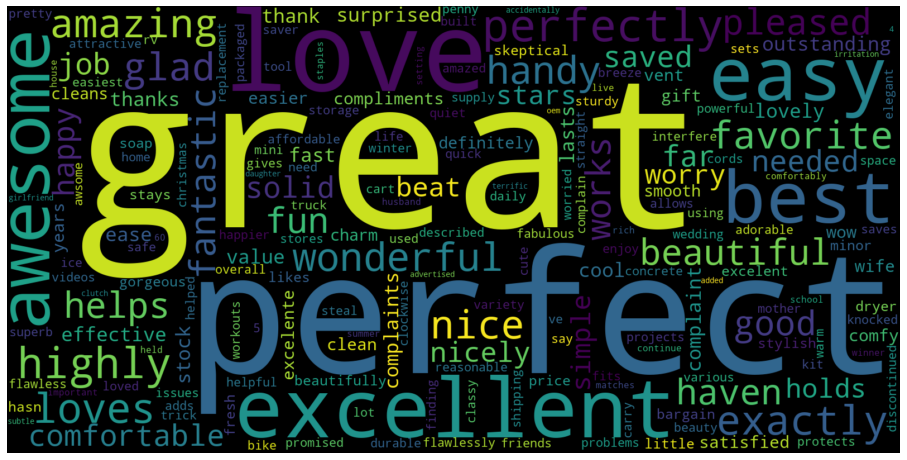
\includegraphics[width=0.9\columnwidth]{word-cloud.png}}
\caption{Word cloud of most sentimentally indicative words.}
\label{fig}
\end{figure}
\FloatBarrier

Fig. 7 shows a word cloud representation of the most indicative features. The size of each word/feature has a direct correlation with the weight assigned to that word by the classification algorithm. For this specific word cloud we used TFIDF stemmed filtered variation with a logistic regression algorithm. It clearly states that the most indicative words in the project are the positive words and this reflects the nature of the dataset.

\begin{figure}[htbp]
\centerline{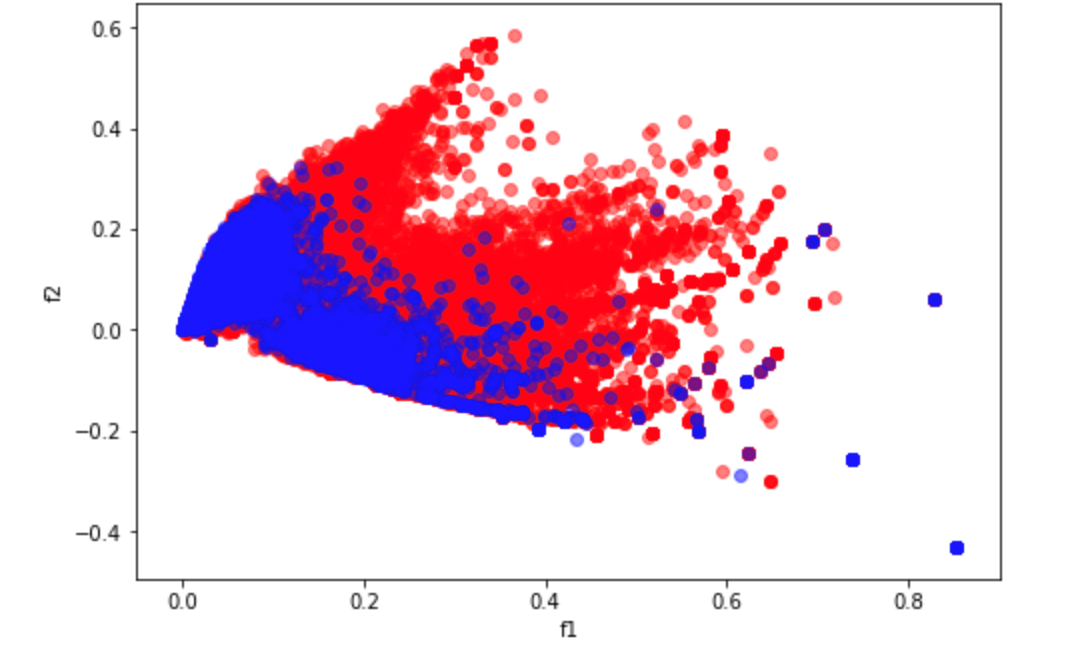
\includegraphics[width=0.9\columnwidth]{pca.png}}
\caption{Principal component analysis Filtered-Stemmed-BOW features.}
\label{fig}
\end{figure}
\FloatBarrier
In order to visualize the data, a scatter plot was created with points categorized with 2 colors (red for positive and blue for negative data points). Since there were a huge number of features involved with the model, PCA was applied. The scatter plot is based on the top two principal components after applying PCA. There was no clear decision boundary dividing the two classes which indicates the complexity of the model. After taking the top three components and creating a 3D scatter plot there still was not any clear hyper plane that would give us two distinct classes.

\section{Future Work}
If the project was to be continued there could be an effective and useful approach to handle the three star reviews and that would be introducing another class such as a neutral review class, for classification of reviews that do not fit in any of the positive or negative classes. This multi-classification approach would need a much more complex preprocessing, since in some instances the data needs to have a neutral label and currently the ratings are the main source of input for assigning a truth label to the data points. Another way this project could be improved is if Neural Networks were used in addition to the main machine learning algorithms discussed in this paper. Traditionally, recurrent neural networks were used for natural language processing projects and machine classification problems that had text as input data. Another idea could be assigning a positive (or negative) label to all of the three star reviews in the preprocessing stage. 


\section{Implementation and Code}



\begin{thebibliography}{00}
\bibitem{b1} Rathor, A. S., Agarwal, A., \& Dimri, P. "Comparative Study of Machine Learning Approaches for Amazon Reviews.” 2018.
\bibitem{b2} Jianmo Ni, Jiacheng Li, Julian McAuley. "Justifying recommendations using distantly-labeled reviews and fined-grained aspects." Empirical Methods in Natural Language Processing (EMNLP), 2019. 
\bibitem{b3} Bing Liu. "Opinion Mining." Invited contribution to Encyclopedia of Database Systems, 2008.
\bibitem{b4} \url{https://www.nltk.org/howto/stem.html}
\bibitem{b5} \url{https://www.cs.uic.edu/~liub/FBS/sentiment-analysis.html#lexicon}
\bibitem{b6} \url{https://www.nltk.org/api/nltk.sentiment.html}
\end{thebibliography}
\end{document}
